\chapter{Experimental Results}
\label{chap:experimental-results}

In this chapter, we evaluate and compare the synthesizers presented in
Chapter~\ref{chap:synthesis}.
The synthesizers are compared in terms of their running time and number of
solved problems.
A description of the benchmarks is provided in Section~\ref{sec:bench-desc}.
Section~\ref{sec:results} presents the results of the benchmarks
and a comparison between the setwise synthesizer
(Section~\ref{sec:setwise-encoding}) and the whole synthesizer
(Section~\ref{sec:whole-encoding}).

\section{Benchmark Description}
\label{sec:bench-desc}

A set of 285522 expressions were provided by OutSystems.
We conducted an analysis to determine which builtin functions and which
combinations were the most common in that set.
We picked 51 expressions containing only those functions (see
Table~\ref{table:builtin-description}) with sizes (number of components) ranging
from 1 to 7.
A description of these 51 expressions in terms of size is shown in
Figure~\ref{fig:bar-chart-sizes-51}.

\begin{figure}
  \centering
  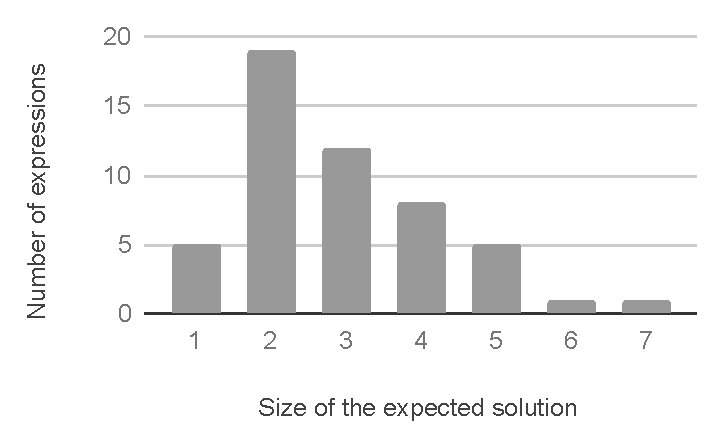
\includegraphics[width=0.5\textwidth]{assets/bar-chart-sizes-51.pdf}
  \caption{Number of expressions per size. For example, there are 31
    expressions of size 2, and 16 expressions of size 1, out of 51 expressions.}
  \label{fig:bar-chart-sizes-51}
\end{figure}

The hardness of a benchmark depends on the size of the solution, the number of
input-output examples, and the library of components.
Typically, the higher the size and the number of components, the harder it is to
synthesize a program.
% Moreover, a library containing components which must be encoded to recursive
% formulas (\lstinline{Replace}, \lstinline{ToLower}, \lstinline{ToUpper},
% \lstinline{Trim}, \lstinline{TrimStart}, and \lstinline{TrimEnd}) makes the
% synthesis problem much harder than if we just had a library whose components
% had a direct counterpart in some \gls{smt} theory.
Figure~\ref{fig:bar-chart-components-freq-51} shows in how many expressions each
component occurs.

\begin{figure}
  \centering
  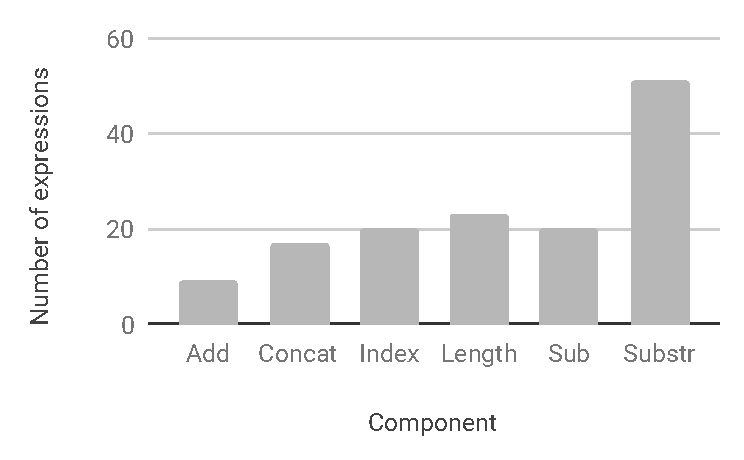
\includegraphics[width=0.5\textwidth]{assets/bar-chart-components-freq-51.pdf}
  \caption{Number of expressions per component.}
  \label{fig:bar-chart-components-freq-51}
\end{figure}

We obtained a set of 3 input-output examples for each of these 51 expressions.
In order to do that, we developed an \textit{interpreter} for OutSystems
expressions, and manually created a set of 3 different inputs for each
expression.
The inputs were carefully crafted in order to try to eliminate as much ambiguity
as possible.
Then we interpreted the expressions over their set of inputs in order to
obtain the correspondent outputs.
A first approach was tried, where we encoded the expressions in \gls{smt} in
such a way that a solution to the formulas yielded valid input-output examples.
Although the approach ``worked'', it was ultimately too slow, and the
automatically generated examples were not natural, so we resorted to the manual
approach.

The \gls{smt} solver used to solve the formulas generated in the synthesis
process was Z3 version 4.8.5~\cite{DeMoura:2008:ZES}.
Each benchmark was monitored by the \textit{runsolver}
program~\cite{Roussel:2011:JSAT}, and restricted to a wall-clock time limit of
10 minutes, and a memory limit of 16 GB.

\section{Results}
\label{sec:results}

We are interested in the relation between the number and quality of the
input-output examples, and their impact on synthesis time and program quality.
In this section, we only study the impact of the number of input-output
examples.

We present the results for both synthesizers discussed in
Chapter~\ref{chap:synthesis} with the following configurations.
For each instance of 3 input-output examples we ran both synthesizers using 1,
2, or all 3 of the input-output examples.
We ran the Setwise synthesizer (Section~\ref{sec:setwise-encoding}) configured
to synthesize programs with a maximum of one integer and one string constants
(configurations S-e1:c1, S-e2:c1, and S-e3:c1, for 1, 2, and 3 input-output
examples, respectively).
We ran the Whole synthesizer (Section~\ref{sec:whole-encoding}) configured to
synthesize programs with a maximum of one constant, which the synthesizer can
choose whether it is a an integer or a string (configurations W-e1:c1, W-e2:c1,
and W-e3:c1, for for 1, 2, and 3 input-output examples, respectively).
Ideally, we would also have tried other configurations to see the impact of
using different number of constants.
For comparison, we also instantiated SyPet~\cite{Feng:2017:CSC}, a
\gls{pbe} component-based synthesizer for Java programs that employs a
type-directed search together with a constraint-based technique, with our
library of components.
However, SyPet does not support guessing the value of constants.
With this in mind, we set up two configurations for SyPet.
For the first configuration (SyPet-All), we introduced a new 0-arity component
for each constant in a pool of predefined constants.~\footnote{The pool of
constants, 43 in total, is the following: \lstinline{0, 1, 2, 3, 4, 5, 6, 7, 8,
9, 10, 15, 16, 20, 30, 40, 50, 60, 70, 80, 90, 100, "", "...", "/", "\", " ",
"-", ".", "@", "," "_","#","(",")","|","<",">",":","Created on ", "updated on",
"\\", " At:". These were chosen in order to roughly match those found in the
expected solutions. The expected solutions employ a total of 34 constants from
this pool.}}
For the second configuration (SyPet-User), we looked at each particular
instance, and introduced new components only for the constants needed for the
expected solution.
This mimics a setting where the constants are declared by the user, instead of
being guessed by the synthesizer.
Both Sypet-User and Sypet-All are configured for using all three examples of
each benchmark, and may use as many constants as they need (out of the available
ones).
Table~\ref{table:comparison-configs} shows a comparison between the different
configurations by number of instances solved and running wall-clock time (mean
and median for solved instances).
An instance is considered solved if the synthesized program satisfies the
input-output examples (but might or might not generalize).
Matching the expected solution means, that the synthesizer outputs a program
that, not only satisfies the input-output examples, but also captures the
original intent and generalizes to more examples.
Figure~\ref{fig:bar-chart-solved-setwise}, shows the number of solved instances
per size of the expected solution for the configurations S-e1:c1, S-e2:c1, and
S-e3:c1.
Figure~\ref{fig:bar-chart-solved-whole} shows the same for configurations
W-e1:c1, W-e2:c1, and W-e3:c1.
Figure~\ref{fig:bar-chart-expected-setwise} shows the number of solved instances
matching the expected solution per size of the expected solution for
configurations S-e1:c1, S-e2:c1, and S-e3:c1.
Figure~\ref{fig:bar-chart-expected-whole} shows the same for configurations
W-e1:c1, W-e2:c1, and W-e3:c1.
Figures~\ref{fig:comparison-solved-sypet} and
\ref{fig:comparison-expected-sypet} show a comparison between all configurations
on three input-output examples.

\begin{table}[]
  \noindent\makebox[\textwidth]{
    \begin{tabular}{ccccc}
      \toprule

      \multicolumn{1}{l}{Configuration}
      & \multicolumn{1}{l}{\# Instances solved}
      & \begin{tabular}[c]{@{}c@{}}\# Instances solved\\ (matching expected\\ solution)\end{tabular}
      & Mean Time (s)
      & \multicolumn{1}{l}{Median Time (s)}
      \\ \midrule

      S-e1:c1    & 48 & 3  & 4.62  & 0.48 \\ \midrule 
      S-e2:c1    & 39 & 21 & 51.28 & 3.21 \\ \midrule
      S-e3:c1    & 34 & 23 & 51.38 & 4.47 \\ \midrule
      W-e1:c1    & 47 & 2  & 6.76  & 0.65 \\ \midrule
      W-e2:c1    & 13 & 4  & 11.14 & 2.24 \\ \midrule
      W-e3:c1    & 9  & 5  & 21.45 & 7.48 \\ \midrule
      SyPet-All  & 11 & 6  & 31.27 & 3.00 \\ \midrule
      SyPet-User & 32 & 30 & 52.75 & 5.00 \\ \bottomrule

    \end{tabular}}
  \caption{Comparison between the different configurations by number of instances
    solved and running wall-clock time for solved instances (not necessarily
    matching the expected solution).}
  \label{table:comparison-configs}
\end{table}

% Solved Setwise
\begin{figure}
  \centering
  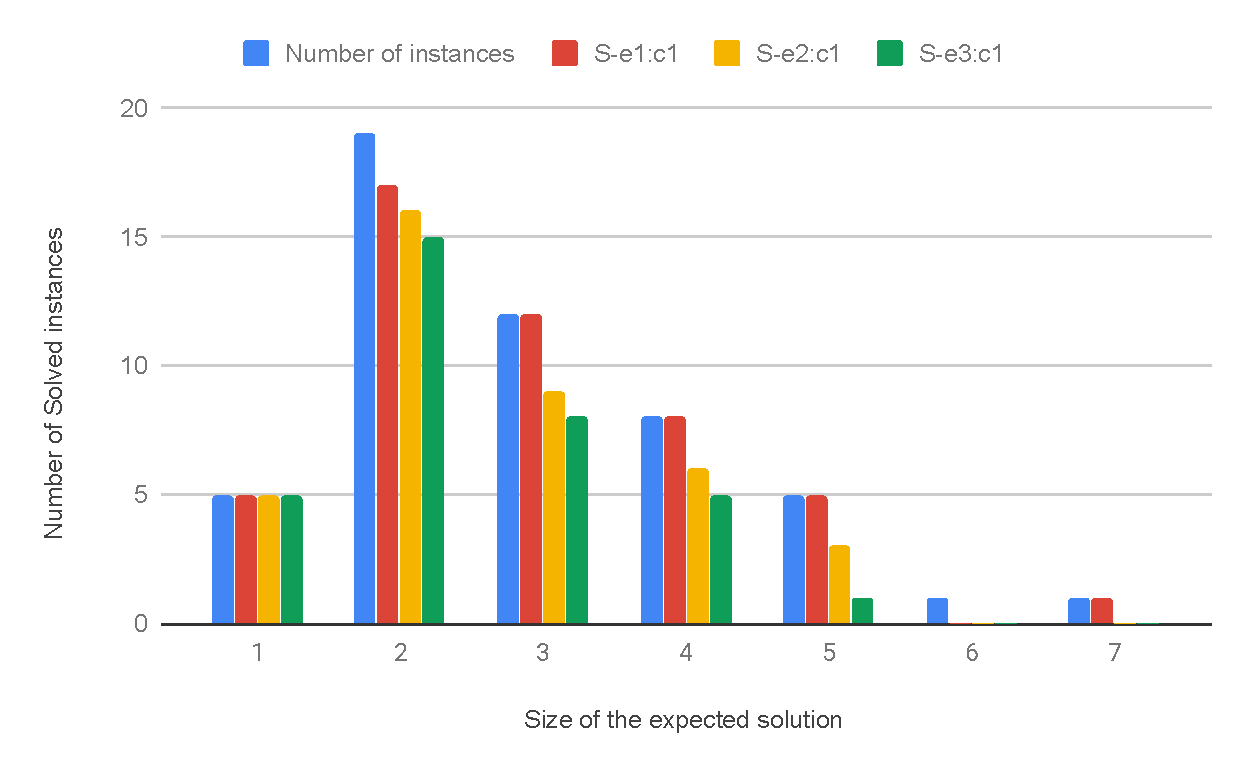
\includegraphics[width=1.0\textwidth]{assets/bar-chart-solved-setwise.pdf}
  \caption{Number of solved instances per size of the expected solution for
    the Setwise synthesizer with one, two, and three examples, one integer
    constant, and one string constant (S-e1:c1, S-e2:c1, S-e3:c1, respectively).}
  \label{fig:bar-chart-solved-setwise}
\end{figure}

% Expected Setwise
\begin{figure}
  \centering
  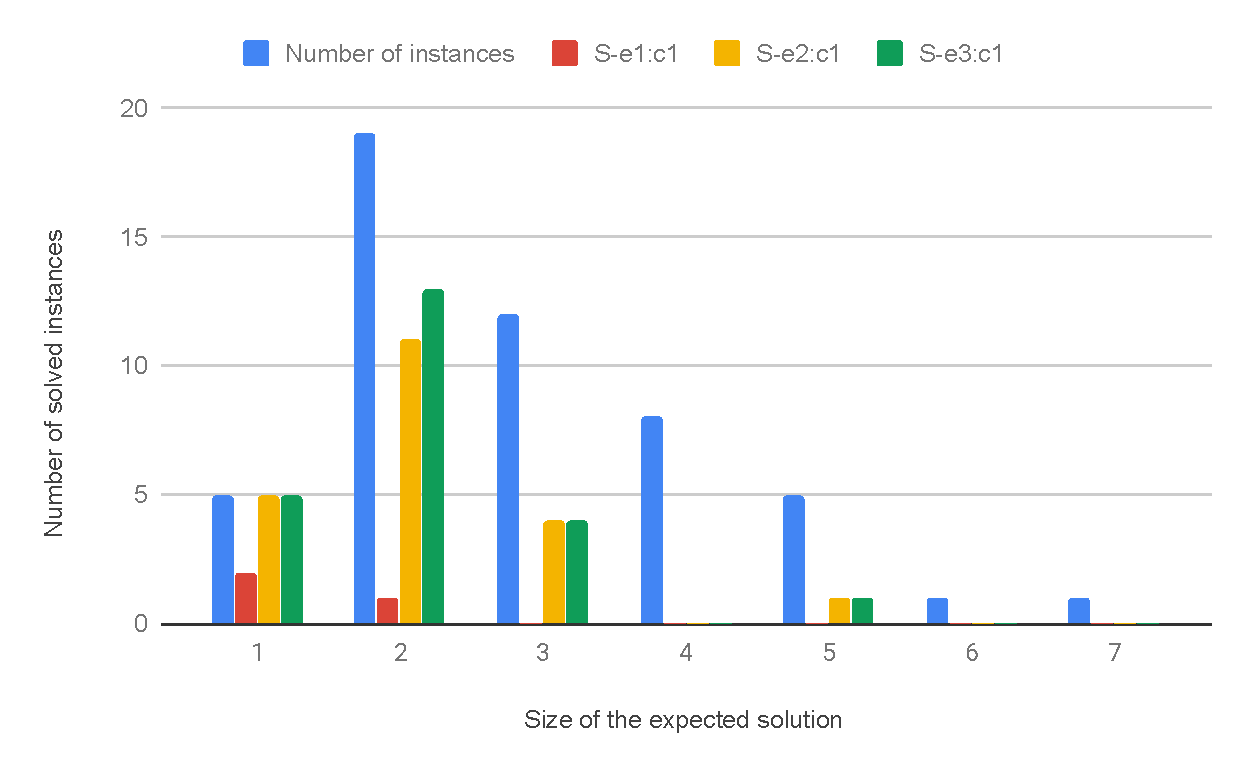
\includegraphics[width=1.0\textwidth]{assets/bar-chart-expected-setwise.pdf}
  \caption{Number of solved instances matching the expected solution per size of
    the expected solution for the Setwise synthesizer with one, two, and three
    examples, one integer constant, and one string constant (S-e1:c1, S-e2:c1,
    S-e3:c1, respectively).}
  \label{fig:bar-chart-expected-setwise}
\end{figure}

% Solved Whole
\begin{figure}
  \centering
  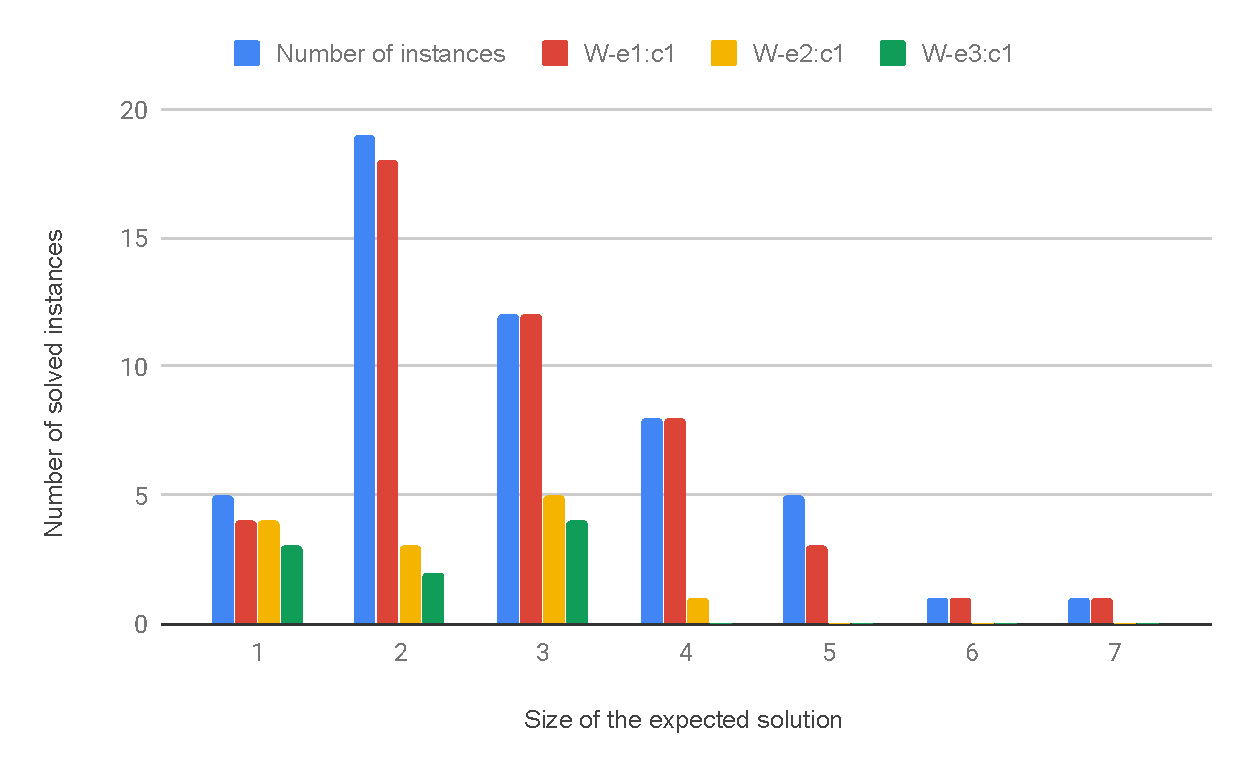
\includegraphics[width=1.0\textwidth]{assets/bar-chart-solved-whole.pdf}
  \caption{Number of solved instances per size of the expected solution for
    the Whole synthesizer with one, two, and three examples, and one constant
    (W-e1:c1, W-e2:c1, W-e3:c1, respectively).}
  \label{fig:bar-chart-solved-whole}
\end{figure}

% Expected Whole
\begin{figure}
  \centering
  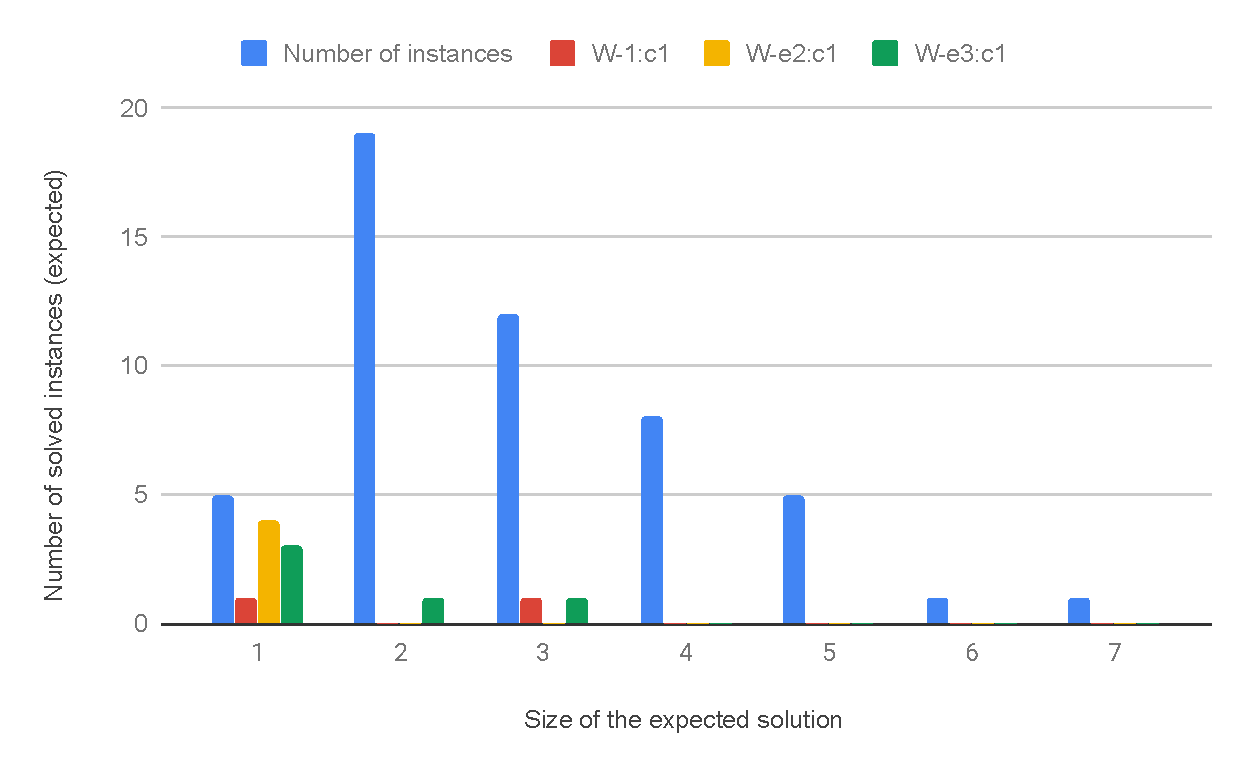
\includegraphics[width=1.0\textwidth]{assets/bar-chart-expected-whole.pdf}
  \caption{Number of solved instances matching the expected solution per size of
    the expected solution for the Whole synthesizer with one, two, and three
    examples, and one constant (W-e1:c1, W-e2:c1, W-e3:c1, respectively).}
  \label{fig:bar-chart-expected-whole}
\end{figure}

% Solved comparison
\begin{figure}
  \centering
  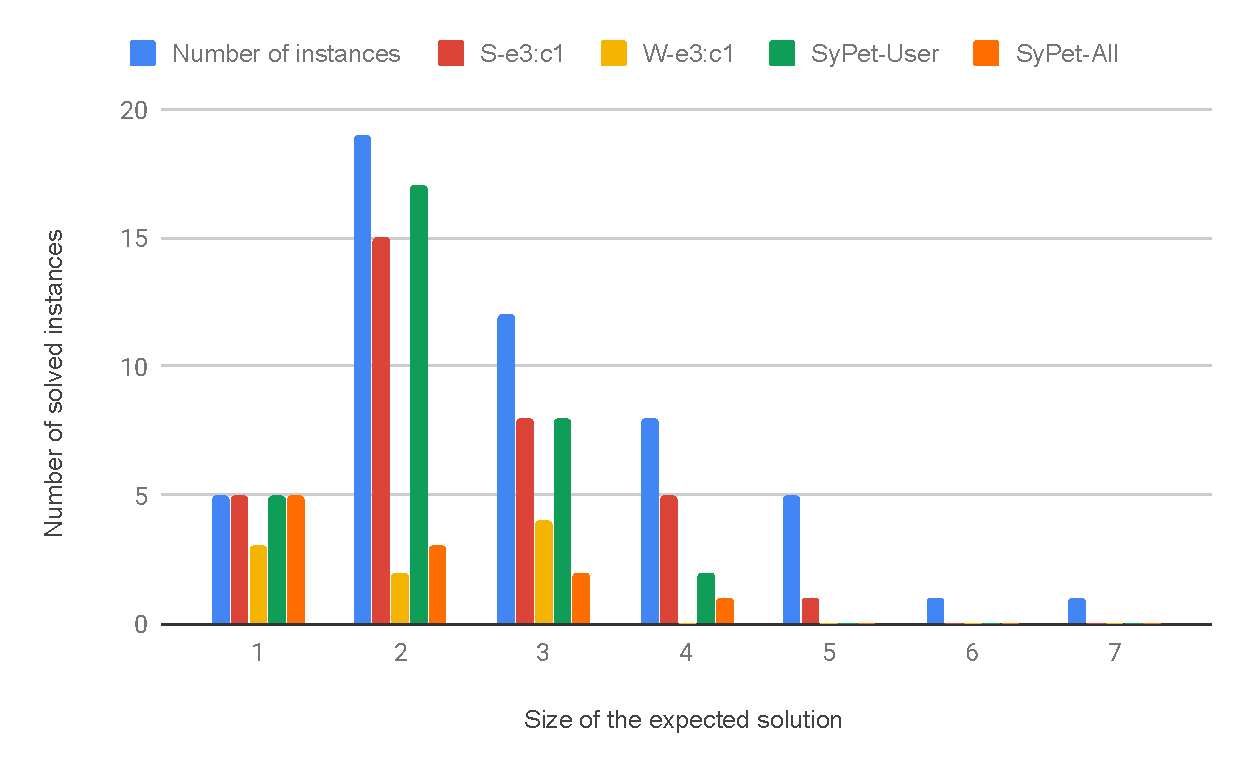
\includegraphics[width=1.0\textwidth]{assets/comparison-solved-sypet.pdf}
  \caption{Number of solved instances per size of the expected solution for the
    Setwise (one integer constant and one string constant) and Whole
    synthesizers (one constant) with three examples, and both SyPet
    configurations (user-provided constants and pool of constants).}
  \label{fig:comparison-solved-sypet}
\end{figure}

% Expected comparison
\begin{figure}
  \centering
  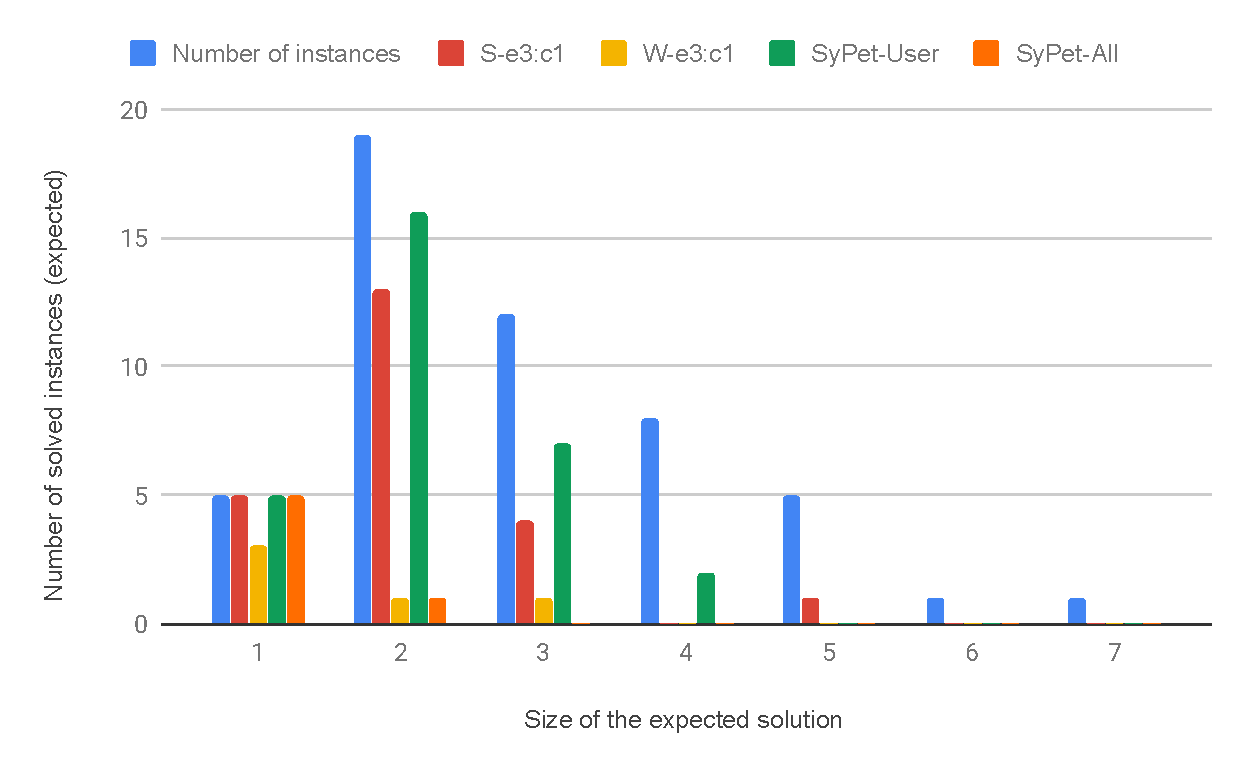
\includegraphics[width=1.0\textwidth]{assets/comparison-expected-sypet.pdf}
  \caption{Number of solved instances matching the expected solution per size of
    the expected solution for the Setwise (one integer constant and one string
    constant) and Whole synthesizers (one constant) with three examples, and
    both SyPet configurations (user-provided constants and pool of constants).}
  \label{fig:comparison-expected-sypet}
\end{figure}

\section{Discussion}
\label{sec:discussion}

Both encodings grow linearly with the number of input-output examples.
Indeed, we can verify that the hardness of the problem increases with the number
of examples (Figures~\ref{fig:bar-chart-solved-setwise},
and~\ref{fig:bar-chart-solved-whole}).
This effect is more evident the more we increase the size of the expected
solution.
On the other hand, the number of programs matching the expected solution should
increase with the number of input-output examples, which we can also verify
(Figures~\ref{fig:bar-chart-expected-setwise}
and~\ref{fig:bar-chart-expected-whole}).
In Figures~\ref{fig:comparison-solved-sypet}
and~\ref{fig:comparison-expected-sypet} we can see that SyPet-All has similar
results to W-e3:c1.
The large number of components makes the search space intractable.
Besides, it cannot take advantage of its type-directed algorithm because we are
dealing with only two types (integers and strings).
This last point also applies to SyPet-User, but the advantage given by the
user-provided constants proves crucial for its fairly good results, which are
actually better than S-e3:c1 (Table~\ref{table:comparison-configs}).

Many expected solutions require more than one constant, with some requiring more
than one constant of each type.
This helps explain the poor performance of the Whole synthesizer.
However, it could be speculated from the start that the Whole synthesizer would
be less efficient than the Setwise synthesizer.
Typically, solving one large constraint is more expensive than solving multiple
smaller constraints.~\footnote{Note that the \gls{smt} problem with the theory
of strings and linear arithmetic is undecidable.}
Still, it would be interesting to benchmark configurations with more
constants, or with user-provided constants.

% Moreover, some more restrictions could be imposed like...

The times for the solved benchmarks are reasonably fast, allowing for reasonable
interaction times with the user.
However, synthesizing programs with 4 or more lines seems to be out of reach for
these configurations (Figure~\ref{fig:comparison-expected-sypet}).
